% !Mode:: "TeX:UTF-8"
\documentclass[type=doctor, openany, pifootnote]{shuthesis}
% 选项:
%  type=[master|doctor],            % 必选
%  secret,                          % 可选 (如果论文需要保密, 这一项需要打开)
%  pifootnote,                      % 可选(建议打开)
%  openany|openright,               % 可选 (章首页是右开还是任意开, 默认是右开)
%  nocolor                          % 提交最终版本时请打开此选项
\usepackage{pdfpages}
\usepackage{shuthesis}
\usepackage{times}
\usepackage{gbt7714}
\bibliographystyle{gbt7714-numerical}
\citestyle{super}                   % 默认引用为角标格式,正文格式为\citestyle{numbers}

\graphicspath{{figures/}}

%\setCJKmainfont{FandolSong-Regular}[BoldFont=FandolHei-Regular,ItalicFont=FandolKai-Regular] % Linux
%\setCJKmainfont{Songti SC Light}[BoldFont=Heiti SC Light,ItalicFont=Kaiti SC, BoldItalicFont=Kaiti SC Bold] % MacOS

% 下面是论文相关信息的填写:
% 论文题目:
\newcommand{\iTitle}{基于摸鱼链的隐私保护摸鱼学习技术研究}
% 学院:
\newcommand{\iSchool}{摸鱼工程与科学学院}
% 专业:
\newcommand{\iMajor}{摸鱼科学与技术}
% 学号:
\newcommand{\iStudentNumber}{20122012}
% 学生姓名:
\newcommand{\iStudentName}{莫雨}
% 指导老师:
\newcommand{\iSupervisorName}{余墨}
% 起讫时间:
\newcommand{\iThesisTime}{2024年1月15日起5月24日止}

\begin{document}
% 第1页:封面页
% !!! 本页不应该做任何修改,相关信息请在 main.tex 填写

\thispagestyle{empty}

\AddToShipoutPictureBG*{%
\AtPageLowerLeft{
\includegraphics[width=\paperwidth,height=\paperheight,keepaspectratio]{figures/cover_background.pdf}}
}
~

\vspace{72pt}

\begin{center}
\chuhao[2]
    本科毕业论文(设计)
\end{center}

\begin{center}
\xiaoer[2]
    UNDERGRADUATE  THESIS (PROJECT)
\end{center}


\begin{table}[h]
\xiaoer[1.5]
\centering
\begin{tabular}{m{4em}<{\centering}m{246pt}<{\centering}}
    \makebox[4em][s]{题\hspace{\fill}目:}  &  {\iTitle} \\ \cline{2-2}
\end{tabular}
\end{table}

\begin{table}[h]
\sanhao[2]
\centering
\begin{tabular}{m{5em}<{\centering}m{246pt}<{\centering}}
    \makebox[5em][s]{学\hspace{\fill}院:}  &  {\iSchool} \\ \cline{2-2}
    \makebox[5em][s]{专\hspace{\fill}业:}  &  {\iMajor} \\ \cline{2-2}
    \makebox[5em][s]{学\hspace{\fill}号:}  &  {\iStudentNumber} \\ \cline{2-2}
    \makebox[5em][s]{学生姓名:}  &  {\iStudentName} \\ \cline{2-2}
    \makebox[5em][s]{指导教师:}  &  {\iSupervisorName} \\ \cline{2-2}
    \makebox[5em][s]{起讫日期:}  &  {\iThesisTime} \\ \cline{2-2}
\end{tabular}
\end{table}

% \begin{table}[]
% \xiaosi[2]
% \begin{tabular}{p{2cm}p{7cm}lll}
% \makebox[5em][s]{姓\hspace{\fill}名:} & {你的名字} & 学号:& {你的学号} &  \\
% \makebox[5em][s]{论文题目:} & \multicolumn{3}{l}{你的论文题目} &  \\
%       &      &         &     &  \\
%       &      &         &     & 
% \end{tabular}
% \end{table}



\vspace{54pt}
\newpage
% 第2页:原创性声明 和 本论文使用授权说明
% !!! 本页不应该做任何修改,相关信息请在 main.tex 填写

\thispagestyle{shu@nopagefoot}


{\xiaosi[2]
\begin{tabular}{p{2cm}p{6.5cm}p{8em}}
\makebox[5em][s]{姓\hspace{\fill}名:} & {\iStudentName} & 学号:~{\iStudentNumber}  \\
\makebox[5em][s]{论文题目:} & \multicolumn{2}{l}{\iTitle}  \\
\end{tabular}}
~

\vspace{22pt}

\begin{center}
    \textbf{\erhao 原~~创~~性~~声~~明}
\end{center}

\vspace{16pt}

{
\sihao[2]
本人声明:所呈交的论文是本人在指导教师指导下进行的研究工作。
除了文中特别加以标注和致谢的地方外,论文中不包含其他人已发表或
撰写过的研究成果。参与同一工作的其他同志对本研究所做的任何贡献
均已在论文中作了明确的说明并表示了谢意。

\vspace{28pt}

签 名:\_\_\_\_\_\_\_\_日 期:\_\_\_\_\_\_\_\_
}

\vspace{14pt}

\begin{center}
    \textbf{\erhao 本论文使用授权说明}
\end{center}

\vspace{16pt}

{
\sihao[2]
本人完全了解上海大学有关保留、使用学位论文的规定,即:学校有权保留论文及送交论文复印件,允许论文被查阅和借阅;学校可以公布论文的全部或部分内容。

\textbf{(保密的论文在解密后应遵守此规定)}

\vspace{28pt}

签 名:\_\_\_\_\_\_\_\_指导教师签名:\_\_\_\_\_\_\_\_日期:\_\_\_\_\_\_\_\_
}
% 如果需要直接覆盖封面和原创性声明,请将下面一行取消注释,并注释上面两行。
% 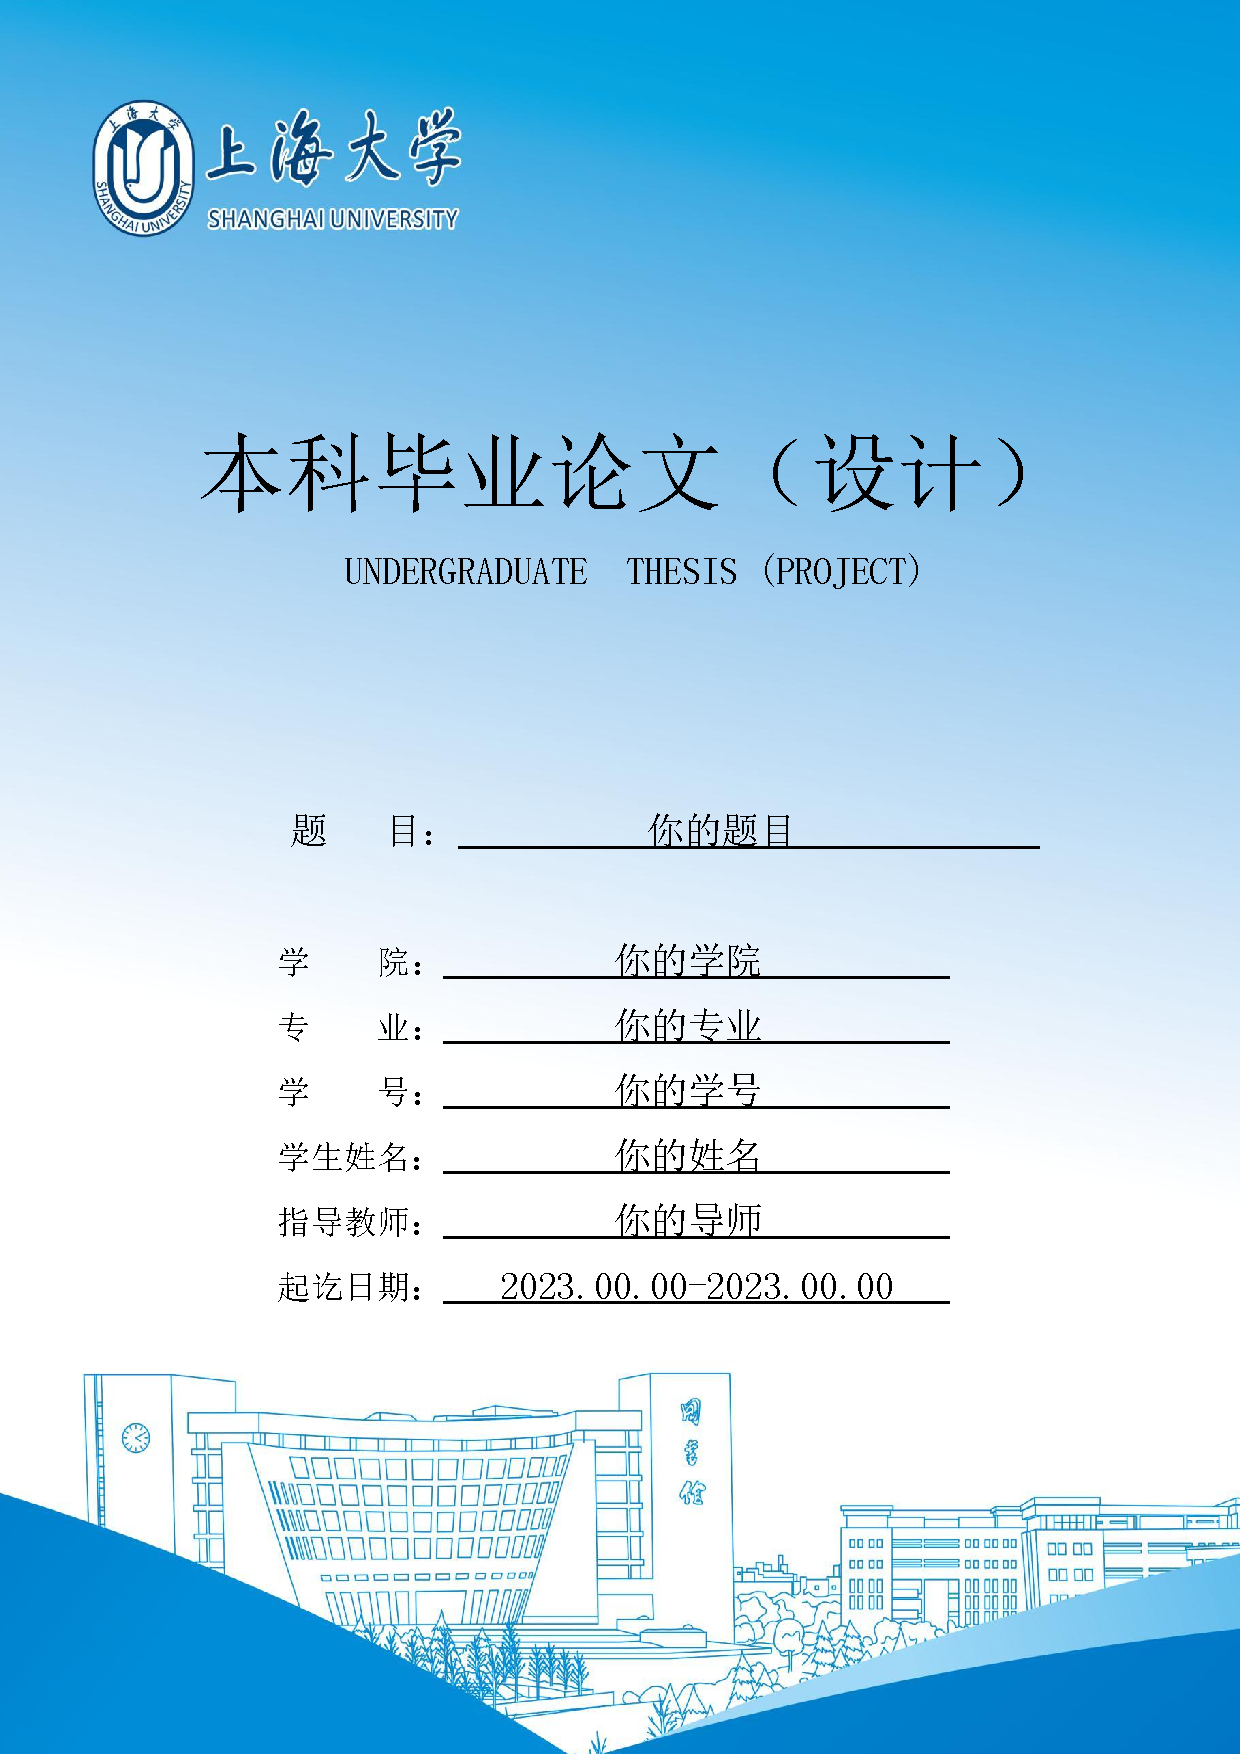
\includepdf[pages={1,2}]{cover.pdf}

\frontmatter
\newpage

{
% \cleardoublepage% Move to first page of new chapter
\let\clearpage\relax% Don't allow page break
\centering\zihao{1}{\textbf{你的文章标题}}

\vspace{8mm}

\chapter*{摘\ 要}
}
\addcontentsline{toc}{chapter}{摘\ 要}

这里是中文摘要。

\vspace{8mm}
\textbf{关键词}: \TeX, \LaTeX, Template, Thesis

\newpage
{
% \cleardoublepage% Move to first page of new chapter
\let\clearpage\relax% Don't allow page break
\centering\zihao{1}{English Title}
\vspace{8mm}

\chapter*{ABSTRACT}
}
\addcontentsline{toc}{chapter}{ABSTRACT}

Abstract in English.

\vspace{8mm}

\textbf{Keywords}: \TeX, \LaTeX, Template, Thesis



{
    \hypersetup{linkcolor=black}
    \tableofcontents
    \thispagestyle{shu@nopagefoot}
}


\mainmatter
% !Mode:: "TeX:UTF-8"
\mychapter{模板介绍}
\label{cha:intro}

\section{\shuthesis 模板(本模板的基模板)介绍}
这是 \shuthesis\ 的示例文档, 基本上覆盖了模板中所有格式的设置. 建议大家在使用模板之
前, 阅读一下 \texttt{shuthesis.pdf} 文档. \shuthesis\ 已经将 \LaTeX 的复杂性尽可
能地进行了封装, 开放出简单的接口, 以便于使用者可以轻易地使用.

\shuthesis\ 是为了帮助上海大学毕业生撰写学位论文而编写的 \LaTeX 模板, 模板的开发
分为两个阶段: 版本 v1.x 是由水寿松制作完成的, 基于 CJK 宏包开发和使用 GBK 编码, 
可在 \url{http://blog.lehu.shu.edu.cn/shuishousong/A209370.html} 下载. 当前
版本是 v2.0, 由 ahhylau 制作完成, 基于 XeCJK 宏包开发, 文件使用 UTF-8 编码. 
\shuthesis\ v2.0 使用文学化编程 (Literate Programming), 利用 \texttt{doc/DocStrip} 
将代码和说明文档混合编写, 便于以后的升级和维护. 另外, 作者重新制作了上海大学 logo 的
高清矢量图, 看起来更加美观. 

目前 \shuthesis\ 模板的代码托管在 \href{https://github.com/ahhylau/shuthesis}{GitHub} 
上, 如有修改建议或者其他要求欢迎在 GitHub 上提交 issue, 作者会尽快回复. 非常期待有其
他上大的 \TeX\ 使用者加入到模板的开发与维护当中来, 不断完善模板.

本模板是以清华大学学位论文模板 \textsc{ThuThesis} 为基础制作的衍生版, 在此对代码的贡
献者表示感谢!

\section{\shubachelorthesisOSC\ 模板}
\shuthesis\ 仅支持硕博论文,后来 \href{https://github.com/alfredbowenfeng}{alfredbowenfeng}
在\shuthesis\ 的基础上修改出了\shubachelorthesis\ ,然而似乎格式和学习官方给出的版本有多处对不上。

因此,我们在 \href{https://github.com/alfredbowenfeng/SHU-Bachelor-Thesis}{\shubachelorthesis\ } 
的基础上进一步制作了上海大学本科生毕业论文Latex模板开源社区版本
\href{https://github.com/EnJiang/SHU-Bachelor-Thesis-OSC}{\shubachelorthesisOSC\ }


感谢前面几位同学的工作和开源精神。希望本模板能帮助到本科生同学,希望越来越多的同学能加入到开源社区大家庭。

\section{目录内容}
模板的源文件即为研究生毕业论文中使用的模板, 用户可以通过修改这些文件来编辑自己的毕业论文.
\begin{itemize}
\item{main.tex}: 主文件, 包含封面部分和基本设置.
\item{data}: 包含本文正文中的所有章节.
\begin{itemize}
\item{abstract.tex}: 中英文摘要.
\item{denotation.tex}: 主要符号对照表.
\item{chap01.tex}: 第一章内容.
\item{chap02.tex}: 第二章内容.
\item{chap03.tex}: 第三章内容.
\item{chap04.tex}: 第四章内容.
\item{acknowledgement.tex}: 致谢.
\item{publications.tex}: 作者在攻读学位期间公开发表的论文.
\item{appendix.tex}: 附录.
\end{itemize}
\item{reference/refs.bib}: 存放论文所引用的全部参考文献信息.
\item{clean.bat}: 双击此文件, 可以用来清理 main.tex 在编译之后生成的所有缓存文件, 
如后缀名为~.aux~,~.log~,~.bak~的文件.
\item{make-doc.bat}: 双击此文件, 一键生成用户手册 \texttt{shuthesis.pdf}.
\end{itemize}


\section{模板使用}
\label{sec:first}

本模板在 Windows 10 和 \TeX Live 2016 下开发, 所使用的宏包均跟进到最新版本. 本模板并
未在其他平台和发行版进行测试, 如 MacOS \& Mac\TeX. 由于历史原因, 目前国内使用 C\TeX\ 
套装的人还是很多. 然而, C\TeX\ 套装自从 2012 年后就不再更新了, 许多宏包已经很老旧了. 
因此从 \shuthesis\ v2.0 开始, 模板不再支持在 C\TeX 套装下使用 (C\TeX\ 2.9.2 及之前
的版本均无法使用). 如果用户需要在 C\TeX\ 下写作, 可使用 \shuthesis\ v1.x. 在 Windows 
系统和 Linux 系统下作者推荐使用 \TeX Live 进行编译; MacOS 系统可使用 Mac\TeX. 











% !Mode:: "TeX:UTF-8"
\chapter{表格和插图}
\label{chap:table} 

\section{表格}
模板中关于表格的宏包有三个: \pkg{booktabs}、\pkg{array} 和 \pkg{longtabular}. 三线表可
以用 \pkg{booktabs} 提供的 \cs{toprule}、\cs{midrule} 和 \cs{bottomrule}. 它们与
\pkg{longtable} 能很好的配合使用.
\begin{table}[htb]
  \centering
  \begin{minipage}[t]{0.8\linewidth} 
  \caption[模板文件]{模板文件}
  \label{tab:template-files}
    \begin{tabularx}{\linewidth}{lX}
      \toprule[1.5pt]
      {\heiti 文件名} & {\heiti 描述} \\\midrule[1pt]
      shuthesis.ins  & \LaTeX{} 安装文件, \textsc{DocStrip}.\footnote{表格中的脚注} \\
      shuthesis.dtx  & 所有的一切都在这里面.\\
      shuthesis.cls  & 模板类文件. \\
      shuthesis.cfg  & 模板配置文.\\
      shuthesis.bst  & 参考文献 BIB\TeX\ 样式文件.\\
      shuthesis.sty  & 常用的包和命令.\\
      \bottomrule[1.5pt]
    \end{tabularx}
  \end{minipage}
\end{table}

\section{插图}
论文里插图可使用 \texttt{graphicx} 宏包. 
\begin{figure}[!htbp]
\centering
\includegraphics[scale=0.3]{shu.pdf}
\caption{上海大学}
\end{figure}

\begin{figure}[!htbp]
\centering
\includegraphics[scale=0.3]{shulogo.pdf}
\caption{上海大学 logo}
\end{figure}

% !Mode:: "TeX:UTF-8"
% Please use \mychapter instead of \chapter
\mychapter{数学和定理环境}
\label{cha:theorem}
\section{数学宏包}
\LaTeX\ 最擅长处理的就是数学公式, \shuthesis\ 已经预加载了常用的数学宏包, 包括:
\begin{itemize}
\item 美国数学学会系列宏包: \texttt{amsmath}, \texttt{amssymb}, \texttt{amsfonts}.
\item 生成英文花体的宏包: \texttt{mathrsfs}.
\item 数学公式中的黑斜体的宏包: \texttt{bm}.
\item AMS 的补充宏包: \texttt{mathtools}.
\end{itemize}

\section{定理类环境}
给大家演示一下 \shuthesis\ 预定义的各种定理类环境.

\subsection{\shuthesis\ 预定义的定理类环境}
\begin{assumption}
天地玄黄, 宇宙洪荒, 日月盈昃, 辰宿列张.
\end{assumption}

\begin{definition}
寒来暑往, 秋收冬藏, 闰余成岁, 律吕调阳.
\end{definition}

\begin{proposition}
云腾致雨, 露结为霜, 金生丽水, 玉出昆冈.
\end{proposition}

\begin{remark}
天不言自高, 水不言自流.
\end{remark}

\begin{axiom}
两点间直线段距离最短.  
\end{axiom}

\begin{lemma}
证明如下等式:
\[
\sum_{n=1}^{\infty}\frac{n-1}{\binom{2n}{n}}=\frac{1}{3}.
\]
\end{lemma}

\begin{proof}
注意到下面的恒等式:
\[
\frac{1}{\binom{2n}{n}}=(2n+1)\int_0^1[x(1-x)]^n\,dx,
\]
和
\[
\sum_{n=1}^{\infty}(2n+1)(n-1)y^n=\frac{(y-5)y^2}{(y-1)^3}.
\]
记 $y=x(1-x)$, 则
\[
\sum_{n=1}^{\infty}(2n+1)(n-1)x^n(1-x)^n=\frac{(x-x^2-5)(x-x^2)^2}{(x-x^2-1)^3}.
\]
所以有
\begin{align*}
\sum_{n=1}^{\infty}\frac{n-1}{\binom{2n}{n}} & =
\int_0^1\left[\sum_{n=1}^{\infty}(2n+1)(n-1)x^n(1-x)^n\right]dx\\
& =\int_0^1\frac{(x-x^2-5)(x-x^2)^2}{(x-x^2-1)^3}dx=\frac13.
\end{align*}
\end{proof}

\begin{theorem}\label{the:theorem1}
一元五次方程没有一般的代数解.
\end{theorem}

\begin{corollary}
这是推论环境.
\end{corollary}

\begin{example}
大家来看一个例子.
\end{example}

\begin{exercise}
设 $a_i\geq0$, $b_i\geq0$, $i=1$, $2$, $\ldots$, $n$, 
且 $p>1$, $q>1$ 满足 $1/p+1/q=1$. 证明
\[
\sum_{i=1}^{n}a_ib_i\leq\left(\sum_{i=1}^{n}a_i^p\right)^{1/p}
\cdot\left(\sum_{i=1}^{n}b_i^q\right)^{1/q},
\]
等号成立当且仅当 $a_i^p=cb_i^q$.
\end{exercise}

\begin{problem}
回答还是不回答, 是个问题. 
\end{problem}

% !Mode:: "TeX:UTF-8"
\chapter{参考文献}
\label{cha:bib}
参考文献可以直接写在 \texttt{thebibliography} 环境里, 利用 \cs{bibitem} 罗列文献条
目. 虽然费点功夫, 但是好控制, 各种格式可以自己随意改写.

本模板推荐使用 BIB\TeX, 样式文件为 \texttt{shuthesis.bst}, 基本符合学校的参考文献格
式. 看看这个例子: 关于书的~\cite{tex1989,algebra2000}, 还有这些\citestyle{numbers} \cite{nikiforov2014,
BuFanZhou2016:Z-eigenvalues,HuQiShao2013:Cored-Hypergraphs,KangNikiforov2014:Extremal-Problems,
LinZhou2016:Distance-Spectral,LuMan2016:Small-Spectral-Radius,Nikiforov2017:Symmetric-Spectrum,
Qi2014:H-Plus-Eigenvalues}.

有时候一些参考文献没有纸质出处, 需要标注 URL. 缺省情况下, URL 不会在连字符处断行,
这可能使得用连字符代替空格的网址分行很难看. 如果需要, 可以将模板类文件中
\begin{verbatim}
\RequirePackage{hyperref}
\end{verbatim}
一行改为:
\begin{verbatim}
\PassOptionsToPackage{hyphens}{url}
\RequirePackage{hyperref}
\end{verbatim}
使得连字符处可以断行. 更多设置可以参考 \texttt{url} 宏包文档.
% !Mode:: "TeX:UTF-8"
\chapter{学校模板提示(正文部分)}

正文是毕业论文的主体和核心部分,不同学科专业和不同的选题可以有不同的写作方式。正文一般包括以下几个方面。

1. 引言或背景

引言是论文正文的开端,引言应包括毕业论文选题的背景、目的和意义;对国内外研究现状和相关领域中已有的研究成果的简要评述;介绍本项研究工作研究设想、研究方法或实验设计、理论依据或实验基础;涉及范围和预期结果等。要求言简意赅,注意不要与摘要雷同或成为摘要的注解。

2. 主体

论文主体是毕业论文的主要部分,必须言之成理,论据可靠,严格遵循本学科国际通行的学术规范。在写作上要注意结构合理、层次分明、重点突出,章节标题、公式图表符号必须规范统一。论文主体的内容根据不同学科有不同的特点,一般应包括以下几个方面:

\begin{enumerate}[(1)]
    \item 毕业设计(论文)总体方案或选题的论证;
    \item 毕业设计(论文)各部分的设计实现,包括实验数据的获取、数据可行性及有效性的处理与分析、各部分的设计计算等;
    \item 对研究内容及成果的客观阐述,包括理论依据、创新见解、创造性成果及其改进与实际应用价值等;
    \item 论文主体的所有数据必须真实可靠,自然科学论文应推理正确、结论清晰;人文和社会学科的论文应把握论点正确、论证充分、论据可靠,恰当运用系统分析和比较研究的方法进行模型或方案设计,注重实证研究和案例分析,根据分析结果提出建议和改进措施等。
\end{enumerate}


3. 结论

结论是毕业论文的总结,是整篇论文的归宿。应精炼、准确、完整。着重阐述自己的创造性成果及其在本研究领域中的意义、作用,还可进一步提出需要讨论的问题和建议。

\begin{conclusion}
  结论是毕业论文的总结,是整篇论文的归宿。应精炼、准确、完整。着重阐
  述自己的创造性成果及其在本研究领域中的意义、作用,还可进一步提出需要讨
  论的问题和建议。
\end{conclusion}
\bibliography{reference/refs}

\backmatter
\begin{appendix}
\chapter{学校模板提示(附录部分)}

论文附录依次用大写字母“附录 A、附录 B、附录 C……”表示,附录内的分级序
号可采用“附 A1、附 A1.1、附 A1.1.1”等表示,图、表、公式均依此类推为“图 A1、
表 A1、式(A1)”等。包含以下内容:

\begin{enumerate}
    \item 代码、图表、标准、手册等数据
    \item 未发表过的一手文献
    \item 公式推导与证明、调查表等
    \item 辅助性教学工具或表格
    \item 其他需要展示或说明的内容
\end{enumerate}

\chapter{经典不等式}
论文中用到的经典不等式.\\

\noindent{\bfseries (H\"older Inequality)}
设~$a_i\geq0$, $b_i\geq0$, $i=1$, $2$, $\cdots$, $n$, 且~$p>1$, $q>1$ 
满足~$1/p+1/q=1$. 则有
\[
\sum_{i=1}^{n}a_ib_i\leq\left(\sum_{i=1}^{n}a_i^p\right)^{\frac1p}
\cdot\left(\sum_{i=1}^{n}b_i^q\right)^{\frac1q},
\]
等号成立当且仅当存在一个常数~$c$ 满足~$a_i^p=cb_i^q$.\\

\noindent{\bfseries (PM Inequality)}
设~$x_1$, $x_2$, $\ldots$, $x_n$ 是~$n$ 个非负实数. 如果~$0<p<q$, 那么
\[
\left(\frac{x_1^p+x_2^p+\cdots+x_n^p}{n}\right)^{\frac{1}{p}}\leq
\left(\frac{x_1^q+x_2^q+\cdots+x_n^q}{n}\right)^{\frac{1}{q}},
\]
等号成立当且仅当~$x_1=x_2=\cdots =x_n$.\\

\noindent{\bfseries (AM-GM Inequality)}
设~$x_1$, $x_2$, $\ldots$, $x_n$ 是~$n$ 个非负实数. 则有
\[
\frac{x_1+x_2+\cdots+x_n}{n}\geq\sqrt[n]{x_1x_2\cdots x_n},
\]
等号成立当且仅当~$x_1=x_2=\cdots =x_n$.
\end{appendix}

% 致谢
\begin{acknowledgement}

    表达真情实感即可。

    衷心感谢导师 xxx 教授对本人的精心指导。
  
    感谢上海大学开源社区提供的 \LaTeX 模板。

    (致谢部分切勿照搬,本部分内容也在论文查重范围之内)

\rightline{作者落款}
\rightline{完成地点}
\rightline{XXXX 年 XX 月 XX 日}

\end{acknowledgement}



\includepdf[pages={1}]{back-cover.pdf}

\end{document}
